\documentclass[tikz,border=4pt]{standalone}
% Paleta y fuentes compartidas por el libro y las figuras (única fuente de verdad).
\RequirePackage{xcolor}
\definecolor{oxido}{HTML}{B7410E}
\definecolor{cobre}{HTML}{D27D2D}
\definecolor{carbon}{HTML}{2B2B2B}
\definecolor{azul}{HTML}{1F5F8B}
\definecolor{arena}{HTML}{F4EDE4}

\usepackage{fontspec}
\setsansfont{FiraSans}[Extension=.otf,UprightFont=*-Regular,BoldFont=*-SemiBold,ItalicFont=*-Italic,BoldItalicFont=*-SemiBoldItalic]
\setmonofont{FiraMono}[Extension=.otf,UprightFont=*-Regular,BoldFont=*-Medium,Scale=0.95]
\usetikzlibrary{positioning,arrows.meta,calc}
\begin{document}
\sffamily\small
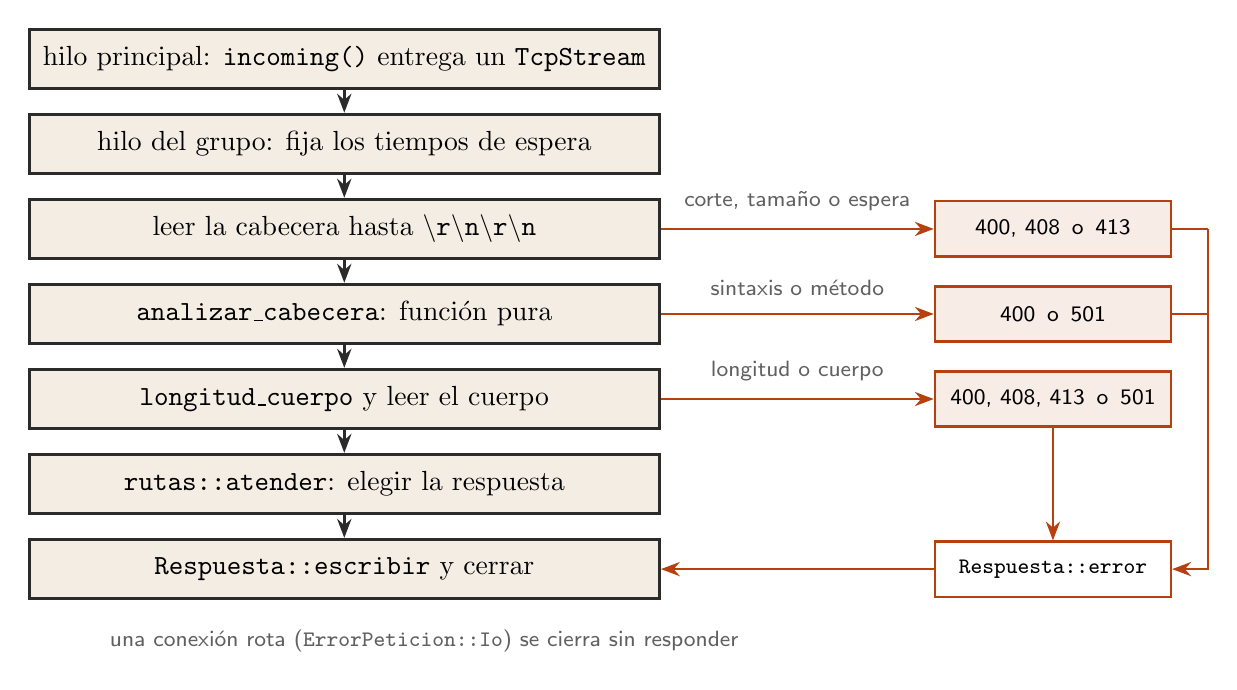
\begin{tikzpicture}[>={Stealth[length=2.4mm]},
  execute at begin node={\hyphenpenalty=10000},
  paso/.style={draw=carbon,very thick,fill=arena,minimum width=80mm,
    minimum height=7.5mm,align=center},
  err/.style={draw=oxido,thick,fill=oxido!10,minimum width=30mm,
    minimum height=7mm,align=center,font=\sffamily\footnotesize},
  rotulo/.style={font=\sffamily\footnotesize,text=carbon!75}]
  \def\dy{1.08}
  \foreach \n/\t [count=\i from 0] in {
    a/{hilo principal: \texttt{incoming()} entrega un \texttt{TcpStream}},
    b/{hilo del grupo: fija los tiempos de espera},
    c/{leer la cabecera hasta \texttt{\textbackslash r\textbackslash n\textbackslash r\textbackslash n}},
    d/{\texttt{analizar\_cabecera}: función pura},
    e/{\texttt{longitud\_cuerpo} y leer el cuerpo},
    f/{\texttt{rutas::atender}: elegir la respuesta},
    g/{\texttt{Respuesta::escribir} y cerrar}} {
    \node[paso] (\n) at (0,-\i*\dy) {\t};
  }
  \foreach \x/\y in {a/b,b/c,c/d,d/e,e/f,f/g} {\draw[->,very thick,carbon] (\x) -- (\y);}
  % Errores
  \def\xe{9.0}
  \node[err] (ec) at (\xe,-2*\dy) {400, 408 \,o\, 413};
  \node[err] (ed) at (\xe,-3*\dy) {400 \,o\, 501};
  \node[err] (ee) at (\xe,-4*\dy) {400, 408, 413 \,o\, 501};
  \foreach \p/\e/\m in {c/ec/{corte, tamaño o espera},d/ed/{sintaxis o método},e/ee/{longitud o cuerpo}} {
    \draw[->,thick,oxido] (\p.east) -- node[rotulo,above=3pt] {\m} (\e.west);
  }
  \node[err,fill=white] (re) at (\xe,-6*\dy) {\texttt{Respuesta::error}};
  \draw[->,thick,oxido] (ee.south) -- (re.north);
  \draw[thick,oxido] (ec.east) -- ++(0.45,0) coordinate (q1);
  \draw[thick,oxido] (ed.east) -- ++(0.45,0);
  \draw[->,thick,oxido] (q1) |- ($(re.east)+(0,0)$);
  \draw[->,thick,oxido] (re.west) -- (g.east);
  \node[rotulo,align=left,anchor=north west] at (-3.1,-6*\dy-0.65)
    {una conexión rota (\texttt{ErrorPeticion::Io}) se cierra sin responder};
\end{tikzpicture}
\end{document}
